\documentclass[runningheads]{llncs}

% ---------------------------------------------------------------
% Include basic ECCV package
 
% TODO REVIEW: Insert your submission number below by replacing '*****'
% TODO FINAL: Comment out the following line for the camera-ready version
\usepackage[review,year=2026,ID=*****]{eccv}
% TODO FINAL: Un-comment the following line for the camera-ready version
%\usepackage{eccv}

% OPTIONAL: Un-comment the following line for a version which is easier to read
% on small portrait-orientation screens (e.g., mobile phones, or beside other windows)
%\usepackage[mobile]{eccv}


% ---------------------------------------------------------------
% Other packages

% Commonly used abbreviations (\eg, \ie, \etc, \cf, \etal, etc.)
\usepackage{eccvabbrv}

% Include other packages here, before hyperref.
\usepackage{graphicx}
\usepackage{booktabs}

% The "axessiblity" package can be found at: https://ctan.org/pkg/axessibility?lang=en
\usepackage[accsupp]{axessibility}  % Improves PDF readability for those with disabilities.


% ---------------------------------------------------------------
% Hyperref package

% It is strongly recommended to use hyperref, especially for the review version.
% Please disable hyperref *only* if you encounter grave issues.
% hyperref with option pagebackref eases the reviewers' job, but should be disabled for the final version.
%
% If you comment hyperref and then uncomment it, you should delete
% main.aux before re-running LaTeX.
% (Or just hit 'q' on the first LaTeX run, let it finish, and you
%  should be clear).

% TODO FINAL: Comment out the following line for the camera-ready version
%\usepackage[pagebackref,breaklinks,colorlinks,citecolor=eccvblue]{hyperref}
% TODO FINAL: Un-comment the following line for the camera-ready version
\usepackage{hyperref}

% Support for ORCID icon
\usepackage{orcidlink}


\begin{document}

% ---------------------------------------------------------------
% TODO REVIEW: Replace with your title
\title{Rethinking Visual Features in Graph-Based Multimodal Emotion Recognition in Conversations (MERC): From Low-Level Pixels to Semantic Representations
}

% TODO REVIEW: If the paper title is too long for the running head, you can set
% an abbreviated paper title here. If not, comment out.
\titlerunning{Abbreviated paper title}

% TODO FINAL: Replace with your author list. 
% Include the authors' OCRID for the camera-ready version, if at all possible.
\author{First Author\inst{1}\orcidlink{0000-1111-2222-3333} \and
  Second Author\inst{2,3}\orcidlink{1111-2222-3333-4444} \and
  Third Author\inst{3}\orcidlink{2222--3333-4444-5555}}

% TODO FINAL: Replace with an abbreviated list of authors.
\authorrunning{F.~Author et al.}
% First names are abbreviated in the running head.
% If there are more than two auGuidelinesthors, 'et al.' is used.

% TODO FINAL: Replace with your institution list.
\institute{Princeton University, Princeton NJ 08544, USA \and
  Springer Heidelberg, Tiergartenstr.~17, 69121 Heidelberg, Germany
  \email{lncs@springer.com}\\
  \url{http://www.springer.com/gp/computer-science/lncs} \and
  ABC Institute, Rupert-Karls-University Heidelberg, Heidelberg, Germany\\
  \email{\{abc,lncs\}@uni-heidelberg.de}}

\maketitle


\begin{abstract}
  Multimodal Emotion Recognition in Conversations (MERC) aims to recognize human emotions for each utterance via visual, audio, and linguistic modalities. Its potential uses in affective computing and human-computer interaction have drawn a lot of attention in recent years. Among the various approaches proposed to solve this problem, graph-based approaches have emerged as some of the most promising ones. However, because this pixel level feature extraction is noisy , the visual modality frequently makes only a small contribution or is underutilized in many graph-based MERC frameworks. Traditional visual encoders generally focus on geometric and textual patterns to produce feature maps or patch representations. These representations often fail to sufficiently express the facial and behavioral cues leading to weak cross-modal alignment with the other semantically rich modalities. To address this problem, we propose a Vision-Language Model (VLM)-based feature extraction approach that captures facial expressions and behavioral cues from the visual modality and encodes them as semantically meaningful representations. Using this approach, the raw video for each utterance is translated into a descriptive and meaningful textual representation through a Vision-Language Model (VLM) with structured prompts designed to capture facial expressions, behavioral cues, and body language. The resulting semantic visual features are then incorporated into graph-based MERC frameworks as a replacement for low-level visual features, reducing noise in the visual modality while increasing the model’s reliance on meaningful visual information through the VLM. This proposed method is expected to solve this problem of underutilization of visual modality while increasing the overall accuracy of MERC.

  \keywords{First keyword \and Second keyword \and Third keyword}
\end{abstract}


\section{Introduction}
\label{sec:intro}

The proper interpretation and communication of emotions are crucial, as they significantly influence interactions, conversations, and decision-making processes. As this modern world advances to an AI dependent future it has become essential to ensure that these emerging AI systems and computers are capable of recognizing emotions at a level comparable to, or exceeding, human ability. But so far understanding human emotions in conversations has been a fundamental challenge in human–computer interaction and affective computing \cite{calvo2010affect}.
Multimodal Emotion Recognition in Conversations (MERC) aims to identify the emotion expressed in each utterance by jointly leveraging information from multiple modalities, typically textual, acoustic, and visual signals \cite{poria2019meld,zadeh2018multimodal}. Unlike traditional single-utterance emotion recognition, MERC must consider contextual dependencies across speakers and time, making it a more complex and realistic setting \cite{majumder2019dialoguernn,ghosal2019dialoguegcn}.Over the past years, numerous approaches have been adopted to solve this problem, starting from early fusion-based techniques and transformer-driven multimodal interaction models to more structured and context-aware graph-based architectures \cite{zadeh2017tfn,tsai2019mult,ghosal2019dialoguegcn,hu2021mmgcn,shou2025comprehensivesurveymultimodalconversational}.
Recent advances have demonstrated that the graph-based architectures, particularly those inspired by Graph Convolutional Networks (GCNs) \cite{kipf2017gcn}, are highly effective for MERC \cite{ghosal2019dialoguegcn,hu2021mmgcn}. By modeling conversational structure as a graph—where utterances are treated as nodes and contextual relationships as edges—these approaches capture both inter-speaker and intra-speaker dependencies \cite{ghosal2019dialoguegcn}. As a result, graph-based MERC models achieve competitive performance on benchmark datasets and are considered among the most promising approaches for conversational emotion recognition \cite{hu2021mmgcn}.

Despite these advances these graph based approaches still face significant problems.One of them is that the visual modality often remains underutilized in many graph‑based MERC frameworks \cite{hu2021mmgcn,li2024graphsmile}. Traditional visual encoders, typically based on convolutional neural networks (CNNs) \cite{he2016resnet} or vision transformers (ViTs) \cite{dosovitskiy2021vit}, extract low-level geometric, texture-based, or patch-level representations from raw video frames. While effective for general visual recognition tasks, these representations often fail to capture subtle behavioral cues and body language that are crucial for emotion understanding \cite{li2018self}. Consequently, the visual modality may contribute less than textual or acoustic modalities, which naturally encode higher-level semantic information \cite{hazarika2018icon}.

Despite advancements, graph-based Multimodal Emotion Recognition in Conversation (MERC) approaches still face significant limitations , one of them being underutilization of a specific modality. Most of the currently existing graph-based MERC frameworks are prone to this limitation underutilizing visual modality while giving priority to the textual modality \cite{hu2021mmgcn,li2024graphsmile}.

Traditional visual encoders relied upon in these baselines, such as Convolutional Neural Networks (CNNs) \cite{he2016resnet} or Vision Transformers (ViTs) \cite{dosovitskiy2021vit}, are fundamentally designed to extract abstract spatial features, structural hierarchies, or patch-level representations from isolated, static video frames. While adequate for general object recognition, these representations create a semantic gap, failing to explicitly capture the subtle behavioral cues, interaction with the other characters in the scene and dynamic body language necessary for complex emotion understanding \cite{li2018self}. Moreover, in standard MERC pipelines, the temporal evolution of emotion within an utterance is largely disregarded. Because graph networks require a fixed-size node representation for structural modeling
\cite{ghosal2019dialoguegcn, hu2021mmgcn}, frame-level visual embeddings are typically aggregated into utterance-level representations via statistical pooling operations, as adopted in multimodal benchmarks \cite{zadeh2018multimodal}. This aggregation effectively collapses the intra-utterance temporal dimension. As a result, dynamic behavioral shifts—such as a speaker transitioning from a frustrated frown to a resigned smile—are mathematically averaged into a single static and potentially emotionally ambiguous feature vector \cite{tsai2019mult}.

Furthermore, real-world conversational videos are prone to noise, including illumination variations, occlusions, and background clutter. This noise severely degrades the quality of pixel-level features. Consequently, the visual modality tends to contribute less to emotion understanding compared to textual or acoustic modalities, which inherently encode higher-level semantic information.

This modality imbalance leads to weak cross-modal alignment in multimodal fusion. Textual features derived from pretrained language models encode high-level semantics \cite{devlin2019bert}, and acoustic features capture prosodic patterns associated with affect \cite{schuller2011recognising}. In contrast, low-level visual embeddings remain largely appearance-based, limiting effective multimodal integration, particularly in graph-based architectures where node representations critically influence relational reasoning \cite{ghosal2019dialoguegcn}.



To address this limitation, we propose rethinking visual feature extraction for graph-based MERC by moving from abstract spatial embeddings to contextualized, semantically meaningful visual descriptions. Specifically, we leverage advanced Video-Language Models—specifically VidEmo-3B, built upon the Qwen2.5-VL-3B architecture \cite{qwen2_5_vl}—which are highly capable of interpreting dynamic visual content and generating temporally grounded semantic representations. Instead of directly feeding mean-pooled, emotionally ambiguous visual vectors into the graph network, we translate each utterance-level video segment into a temporally structured textual narrative. This narrative explicitly tracks the evolution of facial expressions, head movements, and body language from the beginning to the end of the utterance, preserving the critical intra-utterance dynamics that traditional pipelines can not retain.

Through carefully designed prompts, the VLM extracts affect-relevant visual information and encodes it into descriptive semantic representations. These generated textual features serve as high-level visual summaries that are better aligned with linguistic and acoustic modalities \cite{radford2021clip}. The resulting semantic visual features are then integrated into graph-based MERC architectures, replacing traditional low-level visual embeddings. By doing so, we reduce visual noise, improve cross-modal consistency, and encourage the model to rely on meaningful visual signals rather than appearance-based artifacts.

In summary, this work makes the following contributions:

\begin{itemize}
  \item We identify and analyze the underutilization of the visual modality in graph-based MERC frameworks due to noisy and low-level feature representations.
  \item We propose a VLM-based semantic visual feature extraction approach that transforms raw video into structured textual descriptions capturing emotion-relevant cues.
  \item We integrate these semantic visual features into graph-based MERC architectures, promoting stronger cross-modal alignment.
\end{itemize}

By bridging the gap between visual perception and semantic understanding, our approach offers a new direction for enhancing the role of visual information in multimodal conversational emotion recognition.

\section{Methodology}
\label{sec:methodology}

The proposed framework builds upon the GraphSmile architecture~\cite{li2024graphsmile} by introducing a novel approach that converts raw visual inputs into meaningful semantic representations before multimodal fusion.

While prior graph-based Multimodal Emotion Recognition in Conversation (MERC) systems relied on conventional visual encoders---such as DenseNet for extracting abstract spatial features~\cite{huang2017densely} and OpenFace for tracking deterministic facial mechanics like Action Units~\cite{baltrusaitis2018openface}---our methodology moves beyond these restricted appearance descriptors. By leveraging a temporally-aware Vision-Language Model (VLM)~\cite{radford2021clip,qwen2_5_vl}, we encode the rich, semantically grounded behavioral signals present in human speech.

The overall architecture comprises three main stages:
\begin{enumerate}
  \item The independent extraction of utterance-level features across textual, acoustic, and visual modalities.
  \item The construction of multimodal dialogue graphs for alternating propagation via the Graph Structure Fusion (GSF) module~\cite{li2024graphsmile}.
  \item Multitask classification incorporating a Sentiment Dynamics Perception (SDP) module~\cite{li2024graphsmile}.
\end{enumerate}

\subsection{Utterance-Level Feature Extraction}

Each modality is processed independently at the utterance level before being integrated into the multimodal graph.
In contrast to the visual channel, the textual and acoustic modality remains structurally unchanged relative to the GraphSmile baseline~\cite{li2024graphsmile}, preserving a controlled point of comparison.

\subsubsection{Textual Feature Extraction.}
For the textual modality, utterance transcripts are encoded uniformly across both datasets using a pre-trained transformer language model, specifically RoBERTa~\cite{liu2019roberta}. The \texttt{<s>} (classification) token representation of each transcript forms the textual feature vector, $X^t$, capturing lexical and syntactic sentiment signals.

\subsubsection{Acoustic Feature Extraction.}
The acoustic features, $X^a$, capture paralinguistic speech characteristics including fundamental frequency (F0), energy, spectral properties, and temporal statistical functionals that reflect prosody and pitch dynamics. For both the IEMOCAP (6-way)~\cite{busso2008iemocap} and MELD~\cite{poria2019meld} datasets, these utterance-level features are extracted using the openSMILE toolkit with the IS10 configuration~\cite{eyben2010opensmile}.

\subsubsection{Semantic Visual Feature Extraction.}
Traditional visual encoders often fail to fully harness conversational cues because they are restricted to extracting context-blind spatial features or isolated facial mechanics, creating a semantic gap between raw physical movements and complex emotional states. The core methodological contribution addresses this by redefining the visual feature extraction process through a three-stage semantic preprocessing pipeline.

\noindent\textbf{Stage 1: Dataset-Specific Video Preprocessing.}
To ensure the VLM accurately analyzes the correct subject, we apply tailored preprocessing strategies based on the native format of each dataset. The IEMOCAP dataset~\cite{busso2008iemocap}, which consists of continuous, multi-speaker dialogue recordings, undergoes two explicit preprocessing steps. First, the sessions are temporally segmented into discrete, utterance-level clips using provided timestamp annotations; second, each frame is spatially cropped to physically isolate the active speaker and eliminate visual interference. In contrast, the MELD dataset~\cite{poria2019meld} inherently provides pre-segmented utterance-level clips, bypassing the need for physical cropping. Instead, spatial isolation for MELD is achieved entirely through zero-shot prompting, wherein the VLM is explicitly instructed to autonomously identify and focus exclusively on the active speaker within the uncropped, multi-person frame.

\noindent\textbf{Stage 2: VLM Temporal Analysis.}
Each utterance clip is processed by VidEmo-3B (built on the Qwen2.5-VL-3B backbone~\cite{qwen2_5_vl}). The model is driven by a highly structured prompt instructing it to focus exclusively on the active speaker and ignore any other visible participants. The VLM maps the speaker's emotional evolution by dividing the clip into a temporal progression (beginning, middle, and end). For each segment, the model grounds its analysis in specific visible signals across four dimensions:
\begin{itemize}
  \item \textbf{Facial Expressions:} Specific muscle movements of the brow, lips, eyes, jaw, and cheeks.
  \item \textbf{Head \& Gaze:} Tilts, nods, shakes, and eye direction.
  \item \textbf{Body Language:} Posture shifts, gestures, and physical tension or relaxation.
  \item \textbf{Instantaneous Emotion:} The most likely emotional state, explicitly supported by the aforementioned visual cues.
\end{itemize}
The temporal analysis concludes with a one-sentence summary of the overall emotional arc (\eg, \emph{starts neutral $\rightarrow$ builds frustration $\rightarrow$ brief smile at end}). By enforcing that every observation is grounded in a specific visible signal from the speaker, this stage generates a semantically dense, temporally aware description of affective behavior---bypassing the noise of traditional frame-averaging encoders.

\noindent\textbf{Stage 3: Text Encoding of VLM Output.}
To bridge the symbolic output of the VLM with the continuous feature space expected by the graph network, the free-text description is encoded using a pre-trained BERT model~\cite{devlin2019bert}. The resulting fixed-dimensional dense vector serves as the new visual modality feature, $X^v$. Encoding visual behavior in the same semantic space as the transcript fosters superior cross-modal alignment within the GSF module~\cite{li2024graphsmile}.

\section{Initial Submission}

\subsection{Language}
All manuscripts must be in English.


\subsection{Template}
Papers must be prepared with the official LNCS style from Springer.
This applies to both review and camera-ready versions.
Springer requires manuscripts to be prepared in \LaTeX{} (strongly encouraged) or Microsoft Word.

Authors preparing their paper with \LaTeX{} must use the template provided by ECCV, which is based on the corresponding Springer class file \texttt{llncs.cls} but includes line numbers for review (\cref{sec:line-numbering}) and properly anonymizes the paper for review (as in this example document).
Authors who -- for whatever reason -- cannot use \LaTeX{} can alternatively use the official LNCS Word template from Springer.
However, it is the authors' responsibility to ensure that the resulting PDF file is consistent with this example paper and follows it as closely as possible (\ie, includes line numbers, is properly anonymized, \etc).

We would like to stress that the class/style files and the template must not be manipulated and that the guidelines regarding font sizes and format must be adhered to.
For example, please refrain from using any \LaTeX{} or \TeX{} command that modifies the layout settings of the template (\eg, \verb+\textheight+, \verb+\vspace+, \verb+\baselinestretch+, \etc).
Such manual layout adjustments should be limited to very exceptional cases.
This is to ensure that the end product is as homogeneous as possible.

Papers that differ significantly from the required style may be rejected without review.


\subsubsection{Fonts.}
Springer's templates for \LaTeX{} are based on CMR, and the XML templates for Word are based on Times.
We ask you to use the font according to the template used for your papers.
Specifically, please refrain from using Times when preparing your paper with \LaTeX{}.
Using a different font can be interpreted as purposely circumventing the length limitations and may lead to rejection without review.


\subsection{Paper Length}
Papers submitted for review must be complete.
The length should match that intended for final publication.
Papers accepted for the conference will be allocated 14 pages (plus additional pages for references) in the proceedings.
Note that the allocated 14 pages do not include the references.
The reason for this policy is that we do not want authors to omit references for sake of space limitations.

Papers with more than 14 pages (excluding references) will be rejected without review.
This includes papers where the margins and formatting including the font are deemed to have been significantly altered from those laid down by this style guide.

The reason such papers will not be reviewed is that there is no provision for supervised revisions of manuscripts.
The reviewing process cannot determine the suitability of the paper for presentation in 14 pages if it is reviewed in 16.


\subsection{Paper ID}
It is imperative that the paper ID is mentioned on each page of the manuscript of the review version.
Enter your paper ID in the appropriate place in the \LaTeX{} template (see \texttt{\%TODO REVIEW}).
The paper ID is a number automatically assigned to your submission when registering your paper submission on the submission site.


\subsection{Line Numbering}
\label{sec:line-numbering}
All lines should be numbered in the initial submission, as in this example document.
This makes reviewing more efficient, because reviewers can refer to a line on a page.
Line numbering is removed in the camera-ready version.


\section{Policies}
The policies governing the review process of ECCV \ECCVyear{} are detailed on the conference webpage (see \url{ https://eccv.ecva.net/Conferences/2026/SubmissionPolicies}), such as regarding confidentiality, dual submissions, double-blind reviewing, plagiarism, and more.
By submitting a paper to ECCV, the authors acknowledge that they have read the submission policies and that the submission follows the rules set forth.

Accepted papers will be published in LNCS proceedings with Springer.
To that end, authors must follow the Springer Nature Code of Conduct for Authors (see \url{https://www.springernature.com/gp/authors/book-authors-code-of-conduct}).
We would like to draw particular attention to the policies regarding figures and illustrations, as well as ethical approval and informed consent, which are also reproduced on the ECCV website.



\section{Preserving Anonymity}
\label{sec:blind}
ECCV reviewing is double blind, in that authors do not know the names of the area chair/reviewers of their papers, and the area chairs/reviewers cannot, beyond reasonable doubt, infer the names of the authors from the submission and the additional material.
You must not identify the authors nor provide links to websites that identify the authors, neither in the paper nor in the supplemental material.
If you need to cite a different paper of yours that is being submitted concurrently to ECCV, you should \emph{(1)} cite these papers anonymously, \emph{(2)} argue in the body of your paper why your ECCV paper is non-trivially different from these concurrent submissions, and \emph{(3)} include anonymized versions of those papers in the supplemental material.
Violation of any of these guidelines may lead to rejection without review.

Many authors misunderstand the concept of anonymizing for blind review.
Blind review does not mean that one must remove citations to one's own work---in fact it is often impossible to review a paper unless the previous citations are known and available.

Blind review means that you do not use the words ``my'' or ``our'' when citing previous work.
That is all.
(But see below for tech reports.)

Saying ``this builds on the work of Lucy Smith [1]'' does not say that you are Lucy Smith;
it says that you are building on her work.
If you are Smith and Jones, do not say ``as we show in [7]'', say ``as Smith and Jones show in [7]'' and at the end of the paper, include reference 7 as you would any other cited work.

An example of a bad paper just asking to be rejected:
\begin{quote}
  \begin{center}
    An analysis of the frobnicatable foo filter.
  \end{center}

  In this paper we present a performance analysis of our previous paper [1], and show it to be inferior to all previously known methods.
  Why the previous paper was accepted without this analysis is beyond me.

    [1] Removed for blind review
\end{quote}

An example of an acceptable paper:
\begin{quote}
  \begin{center}
    An analysis of the frobnicatable foo filter.
  \end{center}

  In this paper we present a performance analysis of the  paper of Smith \etal [1], and show it to be inferior to all previously known methods.
  Why the previous paper was accepted without this analysis is beyond me.

    [1] Smith, L and Jones, C. ``The frobnicatable foo filter, a fundamental contribution to human knowledge''. Nature 381(12), 1-213.
\end{quote}

If you are making a submission to another conference at the same time, which covers similar or overlapping material, you may need to refer to that submission in order to explain the differences, just as you would if you had previously published related work.
In such cases, include the anonymized parallel submission [1] as supplemental material and cite it as
\begin{quote}
  [1] Authors. ``The frobnicatable foo filter'', ECCV \ECCVyear Submission ID 00324, Supplied as supplemental material {\tt 00324.pdf}.
\end{quote}

Finally, you may feel you need to tell the reader that more details can be found elsewhere, and refer them to a technical report.
For conference submissions, the paper must stand on its own, and not \emph{require} the reviewer to go to a tech report for further details.
Thus, you may say in the body of the paper ``further details may be found in~\cite{Anonymous24b}''.
Then submit the tech report as supplemental material.
Again, you may not assume the reviewers will read this material.

Sometimes your paper is about a problem, which you tested using a tool that is widely known to be restricted to a single institution.
For example, let's say it's 1969, you have solved a key problem on the Apollo lander, and you believe that the ECCV audience would like to hear about your
solution.
The work is a development of your celebrated 1968 paper entitled ``Zero-g frobnication: How being the only people in the world with access to the Apollo lander source code makes us a wow at parties'', by Zeus \etal.

You can handle this paper like any other.
Do not write ``We show how to improve our previous work [Anonymous, 1968].
This time we tested the algorithm on a lunar lander [name of lander removed for blind review]''.
That would be silly, and would immediately identify the authors.
Instead write the following:
\begin{quotation}
  We describe a system for zero-g frobnication.
  This system is new because it handles the following cases:
  A, B.  Previous systems [Zeus et al. 1968] did not  handle case B properly.
  Ours handles it by including a foo term in the bar integral.

  ...

  The proposed system was integrated with the Apollo lunar lander, and went all the way to the moon, don't you know.
  It displayed the following behaviours, which show how well we solved cases A and B: ...
\end{quotation}
As you can see, the above text follows standard scientific convention, reads better than the first version, and does not explicitly name you as the authors.
A reviewer might think it likely that the new paper was written by Zeus \etal, but cannot make any decision based on that guess.
He or she would have to be sure that no other authors could have been contracted to solve problem B.

For sake of anonymity, authors must omit acknowledgements in the review copy.
They can be added later when you prepare the final copy.


\section{Formatting Guidelines}

\subsection{Headings}
Headings should be capitalized (\ie, nouns, verbs, and all other words except articles, prepositions, and conjunctions should be set with an initial capital) and should, with the exception of the title, be aligned to the left.
Only the first two levels of section headings should be numbered, as shown in \cref{tab:headings}.
The respective font sizes are also given in \cref{tab:headings}.
Kindly refrain from using ``0'' when numbering your section headings.
Words joined by a hyphen are subject to a special rule.
If the first word can stand alone, the second word should be capitalized.

\begin{table}[tb]
  \caption{Font sizes of headings.
    Table captions should always be positioned \emph{above} the tables.
  }
  \label{tab:headings}
  \centering
  \begin{tabular}{@{}lll@{}}
    \toprule
    Heading level     & Example                            & Font size and style \\
    \midrule
    Title (centered)  & {\Large\bf Lecture Notes \dots}    & 14 point, bold      \\
    1st-level heading & {\large\bf 1 Introduction}         & 12 point, bold      \\
    2nd-level heading & {\bf 2.1 Printing Area}            & 10 point, bold      \\
    3rd-level heading & {\bf Headings.} Text follows \dots & 10 point, bold      \\
    4th-level heading & {\it Remark.} Text follows \dots   & 10 point, italic    \\
    \bottomrule
  \end{tabular}
\end{table}

Here are some examples of headings:
``Criteria to Disprove Context-Freeness of Collage Languages'', ``On Correcting the Intrusion of Tracing Non-deterministic Programs by Software'', ``A User-Friendly and Extendable Data Distribution System'', ``Multi-flip Networks: Parallelizing GenSAT'', ``Self-determinations of Man''.


\subsection{Figures}
\label{sect:figures}
For \LaTeX{} users, we recommend integrating figures in your paper using the package \texttt{graphicx}.

It is essential that all illustrations are clear and legible.
Vector graphics (rather than rasterized images) should be used for diagrams and schemas whenever possible.
Please check that the lines in line drawings are not interrupted and have a constant width.
Line drawings are to have a resolution of at least 800 dpi (preferably 1200 dpi).
Grids and details within figures must be clearly legible and may not be written one on top of the other.
The lettering in figures should not use font sizes smaller than 6\:pt ($\sim$2\:mm character height).

Figures should be numbered and should have a caption, which should always be positioned \emph{under} the figures, in contrast to the caption belonging to a table, which should always appear \emph{above} the table.
Figures and Tables should be cross-referred in the text.

If they are short, they are centered between the margins (\cf \cref{fig:short}).
Longer captions, covering more than one line, are justified (\cref{fig:example} shows an example).
Captions that do not constitute a full sentence, do not have a period.


\begin{figure}[tb]
  \centering
  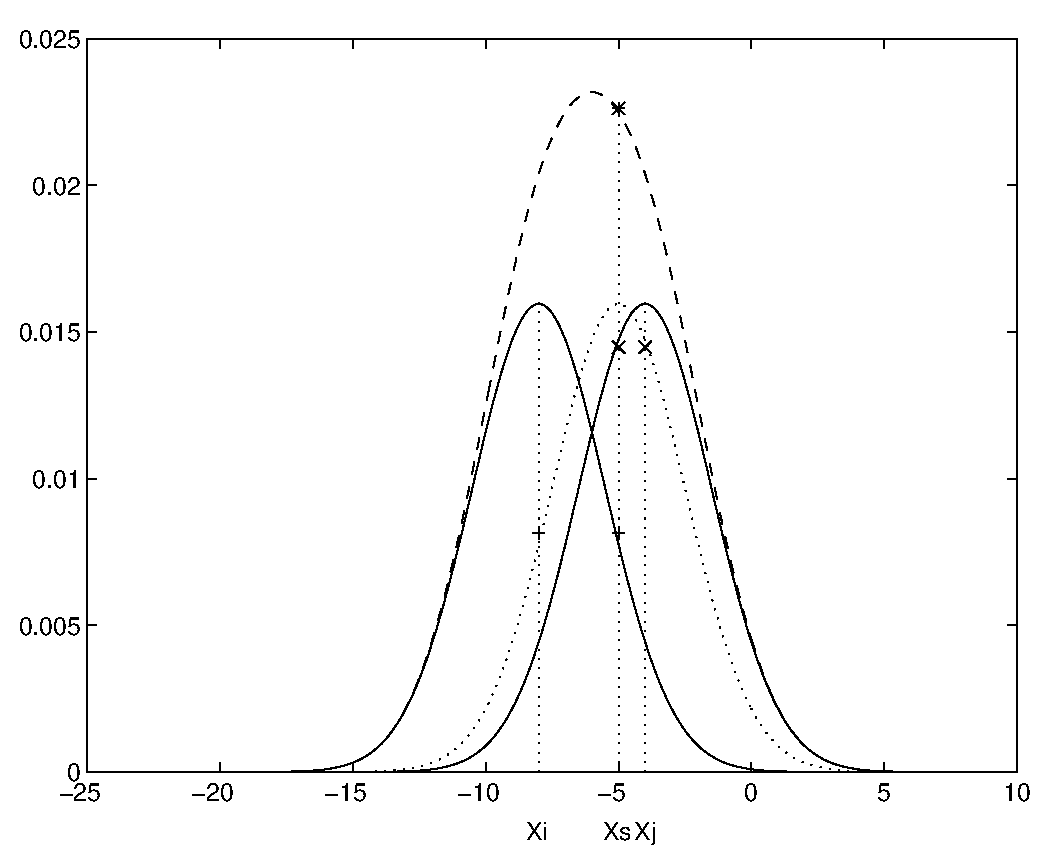
\includegraphics[height=6.5cm]{eijkel2}
  \caption{One kernel at $x_s$ (\emph{dotted kernel}) or two kernels at $x_i$ and $x_j$ (\emph{left and right}) lead to the same summed estimate at $x_s$.
    This shows a figure consisting of different types of lines.
    Elements of the figure described in the caption should be set in italics, in parentheses, as shown in this sample caption.
    The last sentence of a figure caption should generally end with a full stop, except when the caption is not a full sentence.
  }
  \label{fig:example}
\end{figure}

\begin{figure}[tb]
  \centering
  \begin{subfigure}{0.68\linewidth}
    \fbox{\rule{0pt}{0.5in} \rule{.9\linewidth}{0pt}}
    \caption{An example of a subfigure}
    \label{fig:short-a}
  \end{subfigure}
  \hfill
  \begin{subfigure}{0.28\linewidth}
    \fbox{\rule{0pt}{0.5in} \rule{.9\linewidth}{0pt}}
    \caption{Another example of a subfigure}
    \label{fig:short-b}
  \end{subfigure}
  \caption{Centered, short example caption}
  \label{fig:short}
\end{figure}

If possible (\eg, if you use \LaTeX) please define figures as floating objects.
\LaTeX{} users, please avoid using the location parameter ``h'' for ``here''.
If you have to insert a pagebreak before a figure, please ensure that the previous page is completely filled.


\subsection{Formulas}
Displayed equations or formulas are centered and set on a separate line (with an extra line or half line space above and below).
Equations should be numbered for reference.
The numbers should be consecutive within the contribution, with numbers enclosed in parentheses and set on the right margin.
For example,
\begin{align}
  \psi (u) & = \int_{0}^{T} \left[\frac{1}{2}
  \left(\Lambda_{0}^{-1} u,u\right) + N^{\ast} (-u)\right] \text{d}t \; \\
           & = 0
\end{align}
and
\begin{equation}
  E = m\cdot c^2.
  \label{eq:important}
\end{equation}
Please do not include section counters in the numbering.

Numbering equations makes reviewing more efficient, because reviewers can refer to a line on a page.
It is important for readers to be able to refer to any particular equation.
Just because you did not refer to it in the text does not mean some future reader might not need to refer to it.
It is cumbersome to have to use circumlocutions like ``the equation second from the top of page 3''.
(Note that the ruler will not be present in the final copy, so is not an alternative to equation numbers).
All authors will benefit from reading Mermin's description of how to write mathematics:
\url{https://doi.org/10.1063/1.2811173}.

% No color equations in Springer publications.
Equations should never be in color and should be punctuated in the same way as ordinary text.
They should not be pasted in as figures.


\subsubsection{Lemmas, Propositions, and Theorems.}
The numbers accorded to lemmas, propositions, and theorems, \etc should appear in consecutive order, starting with Lemma 1.
Please do not include section counters in the numbering like ``Theorem 1.1''.


\subsection{Footnotes.}
The superscript numeral used to refer to a footnote appears in the text either directly after the word to be discussed or -- in relation to a phrase or a sentence -- following the punctuation mark (comma, semicolon, or period).%
\footnote{The footnote numeral is set flush left and the text follows with the usual word spacing.
  Second and subsequent lines are indented.
}
For remarks pertaining to the title or the authors' names, in the header of a paper, symbols should be used instead of a number.
Please note that no footnotes may be included in the abstract.


\subsection{Cross References}
For the benefit of author(s) and readers, please use the
\begin{verbatim}
  \cref{...}
\end{verbatim}
command for cross-referencing to figures, tables, equations, or sections.
This will automatically insert the appropriate label alongside the cross reference as in this example:
\begin{quotation}
  To see how our method outperforms previous work, please see \cref{fig:example} and \cref{tab:headings}.
  It is also possible to refer to multiple targets as once, \eg~to \cref{fig:example,fig:short-a}.
  You may also return to \cref{sec:intro} or look at \cref{eq:important}.
\end{quotation}
If you do not wish to abbreviate the label, for example at the beginning of the sentence, you can use the
\begin{verbatim}
  \Cref{...}
\end{verbatim}
command. Here is an example:
\begin{quotation}
  \Cref{fig:example} is also quite important.
\end{quotation}


\subsection{Program Code}
Program listings or program commands in the text are normally set in typewriter font (\eg, \texttt{printf("Hello world!\textbackslash{}n");}).


\subsection{Citations}
Arabic numbers are used for citation, which is sequential either by order of citation or by alphabetical order of the references, depending on which sequence is used in the list of references.
The reference numbers are given in brackets and are not superscript.
Please observe the following guidelines:
\begin{itemize}
  \item Single citation: \cite{Anonymous24}
  \item Multiple citation: \cite{Alpher02,Alpher03,Alpher05,Anonymous24b,Anonymous24}.
        The numbers should be listed in numerical order.
        If you use the template as advised, this will be taken care of automatically.
  \item If an author's name is used in the text: Alpher \cite{Alpher02} was the first \ldots
\end{itemize}
Please write all references using the Latin alphabet. If the title of the book you are referring to is, \eg, in Russian or Chinese, then please write (in Russian) or (in Chinese) at the end of the transcript or translation of the title.
All references cited in the text should be in the list of references and vice versa.

References should be formatted with the official LNCS reference style.
The \LaTeX{} template already takes care of that through the use of the \texttt{splncs04.bst} Bib\TeX{} style file.
Springer strongly encourages you to include DOIs (Digital Object Identifiers) in your references (\cf \cite{ECCV2022}).
The DOI is a unique code allotted by the publisher to each online paper or journal article.
It provides a stable way of finding published papers and their metadata.
The insertion of DOIs increases the overall length of the references section, but this should not concern you as the reference section is not counted toward the page limit.


\subsection{Miscellaneous}
Compare the following:
\begin{center}
  \begin{tabular}{ll}
    \verb'$conf_a$'          & $\qquad conf_a$          \\
    \verb'$\mathit{conf}_a$' & $\qquad \mathit{conf}_a$
  \end{tabular}
\end{center}
See The \TeX book, p.\ 165.

The space after \eg, meaning ``for example'', should not be a sentence-ending space.
So \eg is correct, \emph{e.g.} is not.
The provided \verb'\eg' macro takes care of this.

When citing a multi-author paper, you may save space by using ``et alia'',
shortened to ``\etal'' (not ``{\em et.\ al.}'' as ``{\em et\hskip 0.1em}'' is a complete word).
If you use the \verb'\etal' macro provided, then you need not worry about double periods when used at the end of a sentence as in Alpher \etal.
However, use it only when there are three or more authors.
Thus, the following is correct:
``Frobnication has been trendy lately.
It was introduced by Alpher~\cite{Alpher02}, and subsequently developed by
Alpher and Fotheringham-Smythe~\cite{Alpher03}, and Alpher \etal~\cite{Alpher04}.''

This is incorrect: ``... subsequently developed by Alpher \etal~\cite{Alpher03} ...'' because reference~\cite{Alpher03} has just two authors.


\subsection{Most Frequently Encountered Issues}
Please kindly use the checklist below to deal with some of the most frequently encountered issues in the latex files of ECCV submissions.

\begin{itemize}
  \item I have removed all \verb| \vspace| and \verb|\hspace|  commands from my paper.
  \item I have not used \verb|\cite| command in the abstract.
  \item I have entered a correct \verb|\titlerunning{}| command and selected a meaningful short name for the paper.
  \item I have used the same name spelling in all my papers accepted to ECCV and ECCV Workshops.
  \item I have added acknowledgments without a section number, e.g. using the \verb|\section*{}| command.
  \item Excluding references and acknowledgments, my paper is no longer than 14 pages.
  \item I have not decreased the font size of any part of the paper (except tables) to fit into 14 pages, I understand Springer editors will remove such commands.
\end{itemize}


\section{Conclusion}
The paper ends with a conclusion.

\clearpage\mbox{}Page \thepage\ of the manuscript.
\clearpage\mbox{}Page \thepage\ of the manuscript.
\clearpage\mbox{}Page \thepage\ of the manuscript.
\clearpage\mbox{}Page \thepage\ of the manuscript.
\clearpage\mbox{}Page \thepage\ of the manuscript. This is the last page.
\par\vfill\par
Now we have reached the maximum length of an ECCV \ECCVyear{} submission (excluding references and acknowledgements).
References should start immediately after the main text, but can continue past p.\ 14 if needed.
\clearpage  % TODO FINAL: This \clearpage needs to be removed from both review and camera-ready versions.

\section*{Acknowledgements}
Please insert your acknowledgments here.

% ---- Bibliography ----
%
% BibTeX users should specify bibliography style 'splncs04'.
% References will then be sorted and formatted in the correct style.
%
\bibliographystyle{splncs04}
\bibliography{citations,main}
\end{document}
